\documentclass[12pt,a4paper]{article}
\usepackage[utf8]{inputenc}
\usepackage[margin=1in]{geometry}
\usepackage{graphicx}
\usepackage{booktabs}
\usepackage{hyperref}
\usepackage{array}
\usepackage{caption}
\usepackage{float}
\usepackage{longtable}

\begin{document}

% --- TITLE PAGE ---
\begin{titlepage}
    \centering
    \vspace*{1cm}
    
    % Logo Section - Using a fixed size or ratio as per Draft Report.pdf
    
\includegraphics[width=0.45\textwidth]{images/bracu_logo.png} \\
    \vspace{1cm}
    
    % Course Information
    {\large \textbf{CSE461: Introduction to Robotics}} \\
    \vspace{0.5cm}
    {\large Lab Project Report} \\
    
    \vspace{1.5cm}
    
    % Project Title
    {\large \textbf{Title: Smart Follow-Me Shopping Cart (w/ RFID)}} \\
    
    \vspace{1.5cm}
    
    {\large by} \\
    \vspace{0.5cm}
    {\large Group: 06} \\
    {\large Section: 03} \\
    
    \vspace{1cm}
    
    % Group Members Table
    {\large \textbf{Group Members:}} \\
    \vspace{0.5cm}
    \begin{center} % Centers the table specifically
        \begin{tabular}{ll}
            \textbf{Name} & \textbf{ID} \\
            \hline
            Fariha Tanha & 22101296 \\
            Mohammad Jabir Safa Khandoker & 22201108 \\
            Aarya Ibteda Foyez & 22201509 \\
            Mugdha Farheen Kibria & 22299206 \\
            Safwan Masud & 23101425 \\
        \end{tabular}
    \end{center}
    
    \vfill
    
    % Footer Information
    {\large Department of Computer Science and Engineering} \\
    {\large BRAC University} \\
    {\large 4th May 2026}
\end{titlepage}

\newpage

% --- ABSTRACT ---
\section*{Abstract}
This project involves the design and realization of a self-directed autonomous-controlled (AA) Auto-Following Shopping Cart with a built-in RFID/self-checkout system. The overall objective is to attain the retail experience by eradicating the physical burdens of pulling a cart and reducing the time spent talking to a check out until the transaction is finalized. The system is based on a dual-microcontroller setup (Arduino UNO R3 and ESP32) and follows a user using Bluetooth RSSI and avoids obstacles with the help of ultrasonic sensors and using an MPU6050 IMU to minimize the chances of tripping it. At the same time, two built-in RFID RC522 readers, HX711 load cells, enable users to scan items, and monitor their real-time total cost and weight on an LCD display. The small scale implementation of this prototype shows what can be termed as a low-cost and highly effective solution to small retail settings that will foster accessibility of physically impaired and elderly shoppers to the general population; the prototype also serves as a very easy to use budgeting software to the common man. 

\vspace{0.5cm}

\textbf{Keywords:} Robotics, Autonomous Navigation, Embedded Systems, RFID Self-Checkout, Sensor Fusion, Smart Retail.

% --- INTRODUCTION ---
\section{Introduction}
The typical shopping experience in the traditional retail store would include having to manoeuvre their way through packed aisles with overloaded carts, and wait in long check out queues, which would be physically exhausting and time consuming. The aim of the project will be to develop an independent shopping cart robot which will be locked onto a particular user and will follow the user at a safe distance, intelligently avoids any obstacle, and will have an inbuilt self-scan system.The project is a full application of Computer Interfacing and Robotics by combining both SP with wireless communication and user tracking, as well as with the Arduino UNO that provides the ability to control the movement of the SP and monitor the environmental conditions via sensors. The areas of this system are focused on small-to-medium stores and libraries, offering a localized, low-cost solution that can be easily budgeted, provides shopping checklisting, and promotes peace of mind. 


% --- RELATED WORK ---
\section{Related Work/Inspiration}
Recent developments in smart retail have brought about technologies such as the Amazon Dash Cart which uses advanced computer vision, multiple cameras, and heavy processing onboard to track the items. Although very precise, they are very costly that small retail stores cannot afford and come at an enormous price to install infrastructural costs.The reason behind the inspiration of our project is based on these autonomous retail solutions yet adjusts the high cost and complexity problem. Our system based on the localized RFID system in combination with a load cell that would verify the weight and Bluetooth RSSI (Received Signal Strength Indicator) so that the user can be tracked down dramatically reduces the computational burden and in turn the cost of the hardware. This makes our system stand out as a highly scalable, low-cost alternative which nevertheless addresses the fundamental causes of physical strain as well as lengthy checkout lines. 


% --- TECHNICAL APPROACH ---
\section{Technical Approach}
\subsection{System Architecture}
The robot employs a distributed, Master-Slave subsumption architecture to divide computational load and ensure real-time responsiveness.

\begin{itemize}
    \item \textbf{ESP32 (Master - High-Level Logic):} It plays the role of the central command hub. It controls Bluetooth Low Energy (BLE) RSSI tracking, point-of-sale (POS) state machines via the RFID-RC522, verifies the weight through HX711 load cell and the I2C LCD user interface. It also supervises proprioception using the MPU6050 IMU for anti-theft and safety purposes. It computes the important tracking state and conveys formatted UART packets to the subordinate controller.

    \item \textbf{Arduino UNO (Slave - Low-Level Locomotion):} It plays the role of a dedicated hardware coprocessor. Without any break, it  polls a three-directional array of HC-SR04 ultrasonic sensors and outputs hardware PWM to dual L298N motor drivers. ESP32 sends the directives of the movement, received by this component but preserves the authority to outgrow those commands based on instant physical obstacles.
\end{itemize}

\subsection{Components Used}
\begin{itemize}
    \item \textbf{ESP32 DevKit:} Master microcontroller with BLE tracking, RFID POS logic, anti-tip monitoring, and UI updates.
    \item \textbf{Arduino UNO R3:} Slave coprocessor that is specifically used in real-time motor control and ultrasonic obstacle avoidance.
    \item \textbf{Smart Phone:} The smart phone will be used as the Bluetooth Low Energy (BLE) beacon, which the cart constantly tracks to follow the user.
    \item \textbf{Ultrasonic Sensor HC-SR04:} Detects the physical obstacles around it so that it can automatically avoid collisions by detecting an object at the proper location. 
    \item \textbf{MPU6050:} This is an IMU sensor that measures the pitch and roll in order to immediately stop the cart in case it has tipped over at an unsafe angle.
    \item \textbf{RFID Reader RC522:} Will scan the NFC product tags to add or remove to the digital shopping cart inventory.
    \item \textbf{RFID NFC Smart Card:} Is the digital barcode that will be attached to physical products to allow them to be identified by the POS system. 
    \item \textbf{Load cell (10 kg) + HX711:} An electronic scale that will prevent theft by ensuring that the physical weight added matches the weight of the scanned item in the database. 
    \item \textbf{LCD 16x2 with I2C module:}  Display of real-time cart telemetry: Total bill, number of items, strength of the Bluetooth signal.
    \item \textbf{Buttons:}  Intended to be used by the physical user interface to activate the checkout mode, remove items, or empty the cart. 
    \item \textbf{L298N Motor Driver:}  L298N bridges the gap between the logical and the physical worlds, by converting Arduino PWM signals into high-current power to the wheels.
    \item \textbf{DC Gear Motors (4WD) Chassis:} The physical drivetrain and structural frame that provides the torque needed to move the cart.
    \item \textbf{Battery 3.7V:} High-capacity Li-ion cells providing the primary energy source to drive the heavy motors and microcontrollers.
    \item \textbf{Battery case 4xAA:} Holds auxiliary batteries to provide isolated, stable power to sensitive logic boards, preventing motor voltage drops.
    \item \textbf{Power Distribution Board:} Safely routes raw battery voltage into regulated 5V, 3.3V, and 12V outputs for the system's various electronics.
    \item \textbf{Resistors:} Used primarily as a voltage divider to safely step down the Arduino's 5V UART transmission to the ESP32's 3.3V logic limit.
\end{itemize}


\subsection{Cost Breakdown}
\begin{table}[h!]
    \centering
    \begin{tabular}{|l|c|c|c|}
        \hline
        \textbf{Component} & \textbf{Qty} & \textbf{Unit Cost (BDT)} & \textbf{Total (BDT)} \\
        \hline
        Arduino UNO R3 & 1 & 480 & 480 \\
        ESP32 DevKit & 1 & 420 & 420 \\
        Smart Phone & 1 & 0 & 0 \\
        L298N Motor Driver & 2 & 120 & 240 \\
        DC Gear Motors (4WD) Chassis & 1 & 750 & 750 \\
        Ultrasonic Sensor HC-SR04 & 4 & 60 & 240 \\
        MPU6050 & 1 & 160 & 160 \\
        RFID Reader RC522 & 1 & 110 & 110 \\
        RFID NFC Smart Card & 5 & 25 & 125 \\
        Load cell (10 kg) + HX711 & 1 & 220 & 220 \\
        LCD 16x2 with I2C module & 1 & 195 & 195 \\
        Buttons & 2 & 3 & 5 \\
        Battery case 4xAA & 1 & 45 & 45 \\
        Battery 3.7V & 4 & 95 & 380 \\
        Power Distribution Board & 1 & 330 & 330 \\
        Jumper Wires (M-M, M-F, F-F) & 65 & 3 & 195 \\
        Resistors & 50 & 1 & 50 \\
        Breadboards (Small) & 2 & 60 & 120 \\
        Soldering Iron & 1 & 495 & 495 \\
        Soldering Wire & 1 & 210 & 210 \\
        Soldering Rosin & 1 & 20 & 20 \\
        Soldering Stand & 1 & 110 & 110 \\
        \hline
        \textbf{Grand Total} & & & \textbf{4900} \\
        \hline
    \end{tabular}
\end{table}

\newpage

\subsection{Circuit/Schematic Integration}
\begin{figure}[H]
    \centering
    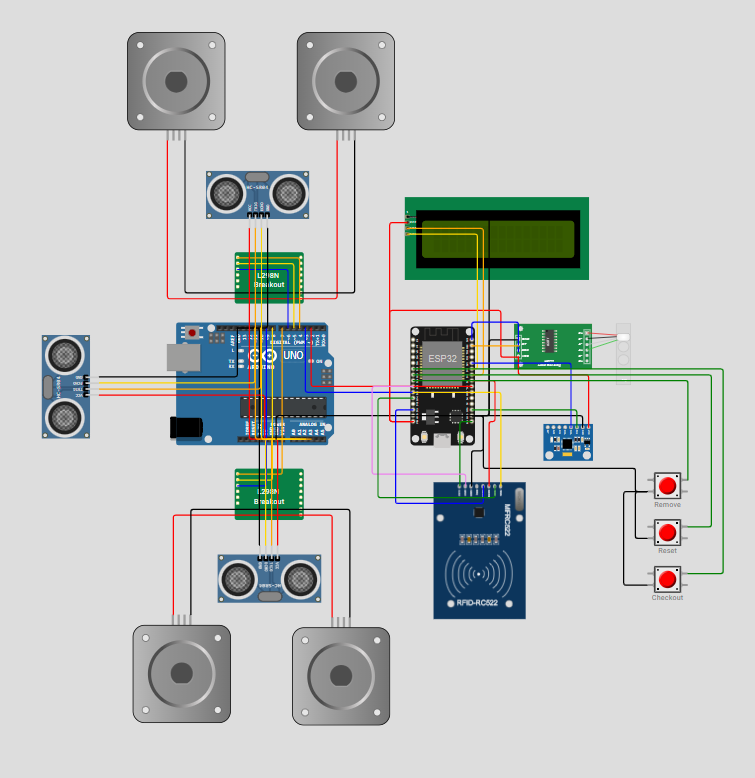
\includegraphics[width=1\linewidth]{images/schematic.png}
    \caption{Pin Configuration of Arduino UNO and ESP32}
    \label{fig:schematic}
\end{figure}

\begin{figure}[H]
    \centering
    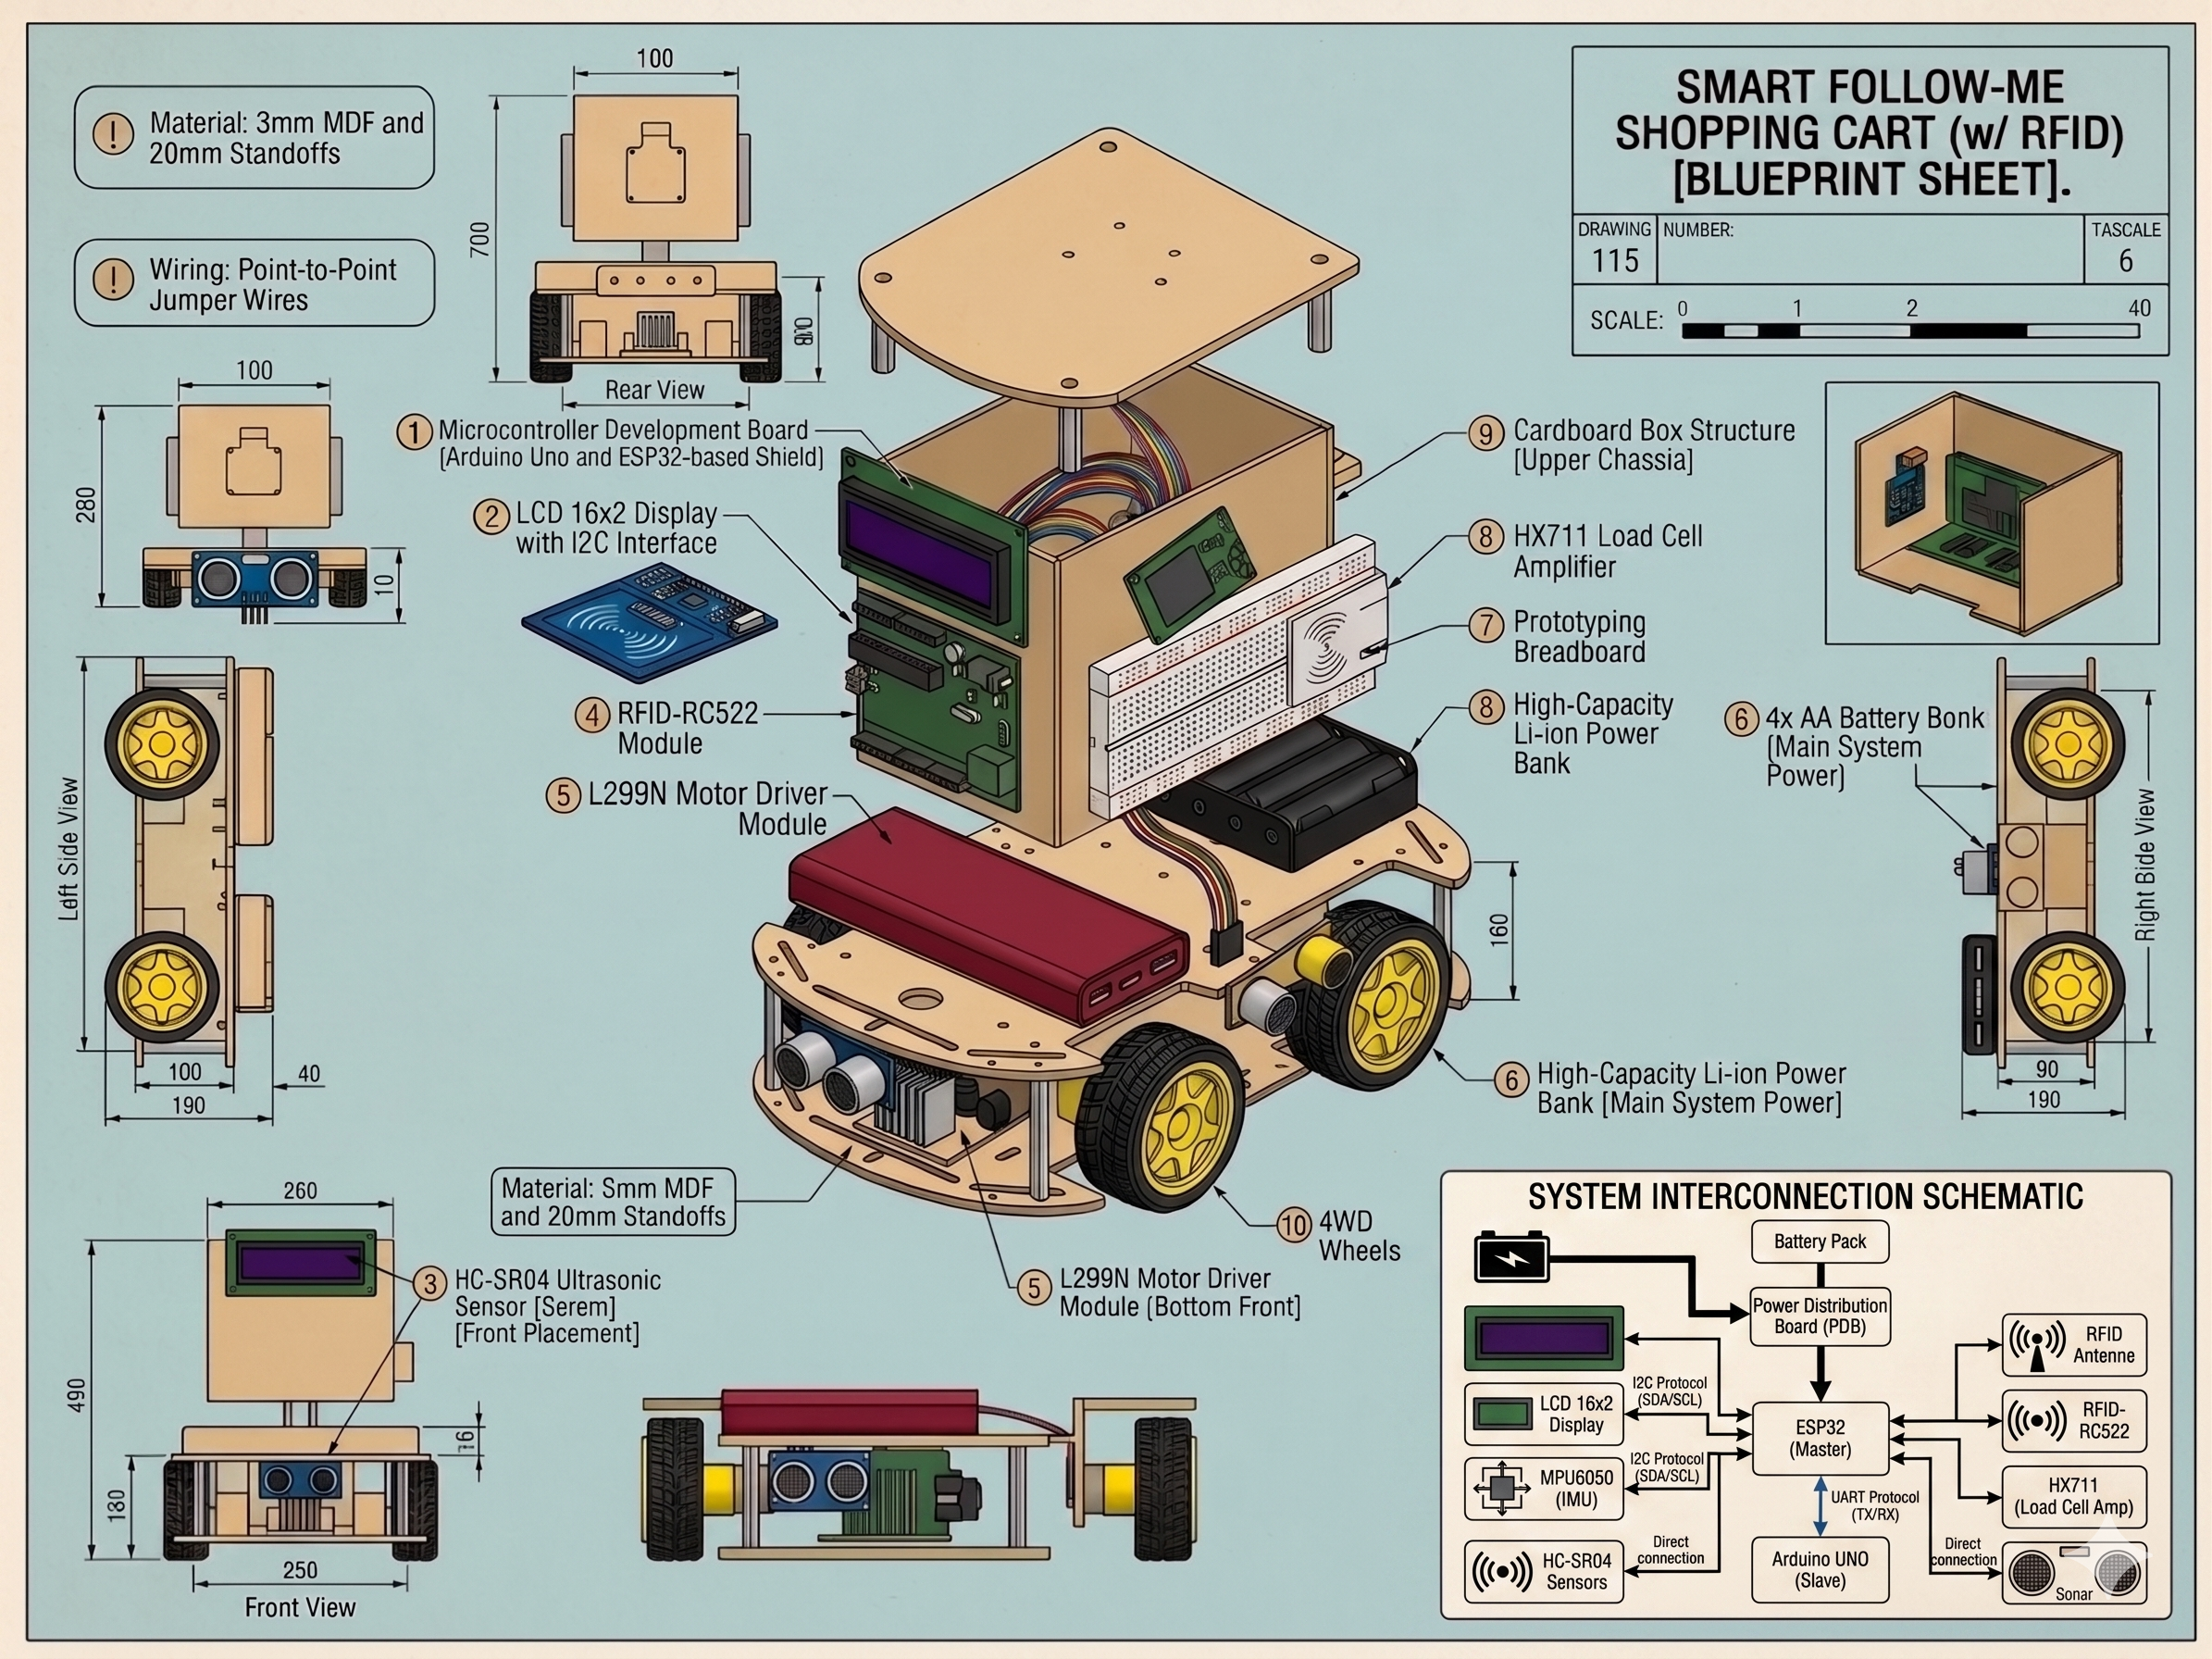
\includegraphics[width=1\linewidth]{images/blueprint.png}
    \caption{Blueprint of the Robot Body}
    \label{fig:blueprint}
\end{figure}

\subsection{ Hardware Integration \& Communication Protocols}
\begin{itemize}
    \item \textbf{Logic Level Shifting:} Because the ESP32 operates at 3.3V logic and the Arduino UNO operates at 5V logic, direct serial communication can cause hardware damage or dropped packets. A bidirectional logic level shifter (or appropriate resistor voltage divider network) is utilized on the UART bridge (ESP32 TX/RX to UNO RX/TX) to ensure safe 9600-baud data transmission.

    \item \textbf{Sensor Buses:} To maximize GPIO efficiency, peripheral communication is heavily multiplexed. The LCD and MPU6050 share the I2C bus (utilizing custom pins 21/15 for the MPU), while the RFID module utilizes a dedicated high-speed SPI bus (Pins 14, 13, 5, 27).

    \item \textbf{Power Distribution:} The system utilizes separated power domains to prevent motor noise from resetting the microcontrollers. Four 3.7V DC Batteries are connected in a serial case to project 14.8V, which has been routed into a Power Distribution Board (PDB). The PDB has 2 built-in Shift Down Voltage Converters, one with 12V and another with 5V as output. The 12V is used to power the L298N Driver Motors and the 4 DC Motors. The 5V is used to power all the other components including the microcontrollers Arduino UNO and ESP32. For safety reasons, the microcontrollers are also powered through a Power Bank. Also, 3 resistors have been used as Voltage Dividers to supply ESP32 with 3.3V during the UART Protocol between Arduino UNO and ESP32.

\end{itemize}

\subsection{Functionality Workflow}
\begin{itemize}
    \item \textbf{User Lock-On \& Proportional Tracking:} The ESP32 utilizes a custom BLE callback to actively scan for a target device (e.g., "CART\_REMOTE"). By calculating the Received Signal Strength Indicator (RSSI), it establishes a tracking "Sweet Spot" ($-50$ dBm to $-85$ dBm). The ESP32 transmits this RSSI value over UART to the UNO, which maps the signal strength to a proportional PWM speed—accelerating when the user pulls away and slowing down as they stop.

    \item \textbf{Subsumption Safety \& Obstacle Avoidance:} The Arduino UNO makes use of a subsumption control loop. Prior to the implementation of any forward tracking command it checks the sonar array. Should an obstacle in front of the sensor be counted as a 30cm threshold is exceeded, the UNO will execute a hard stop and overwrite the ESP32. Should a side obstacle breach the 20cm threshold, it will perform a so-called Soft Nudge, reducing PWM power to only one side, so as to gradually drift away along the wall.

    \item \textbf{Emergency Override (Deadman \& Anti-Tip):} If UNO does not receive any UART packet within 1000ms (a Deadman Switch timeout), it views that there is some problem with the system and it locks the motors. Moreover, when the MPU6050 in the ESP32 detects a tilt of more than $35^{\circ}$ in the X or Y-axis it transmits a $-100$ signal (Lock) to immediately stop the cart and prevent falling over.

    \item \textbf{Interactive POS (Point of Sale):} Once a user touches an RFID product tag, the ESP32 halts all motor tracking to make sure that a safe transaction is made. It also queries the local database and displays the new count of items and the total financial value on the 16x2 LCD display and monitors the HX711 load cell to ensure the real physical weight is the same as the one in the digital database.
\end{itemize}

\begin{figure} [H]
    \centering
    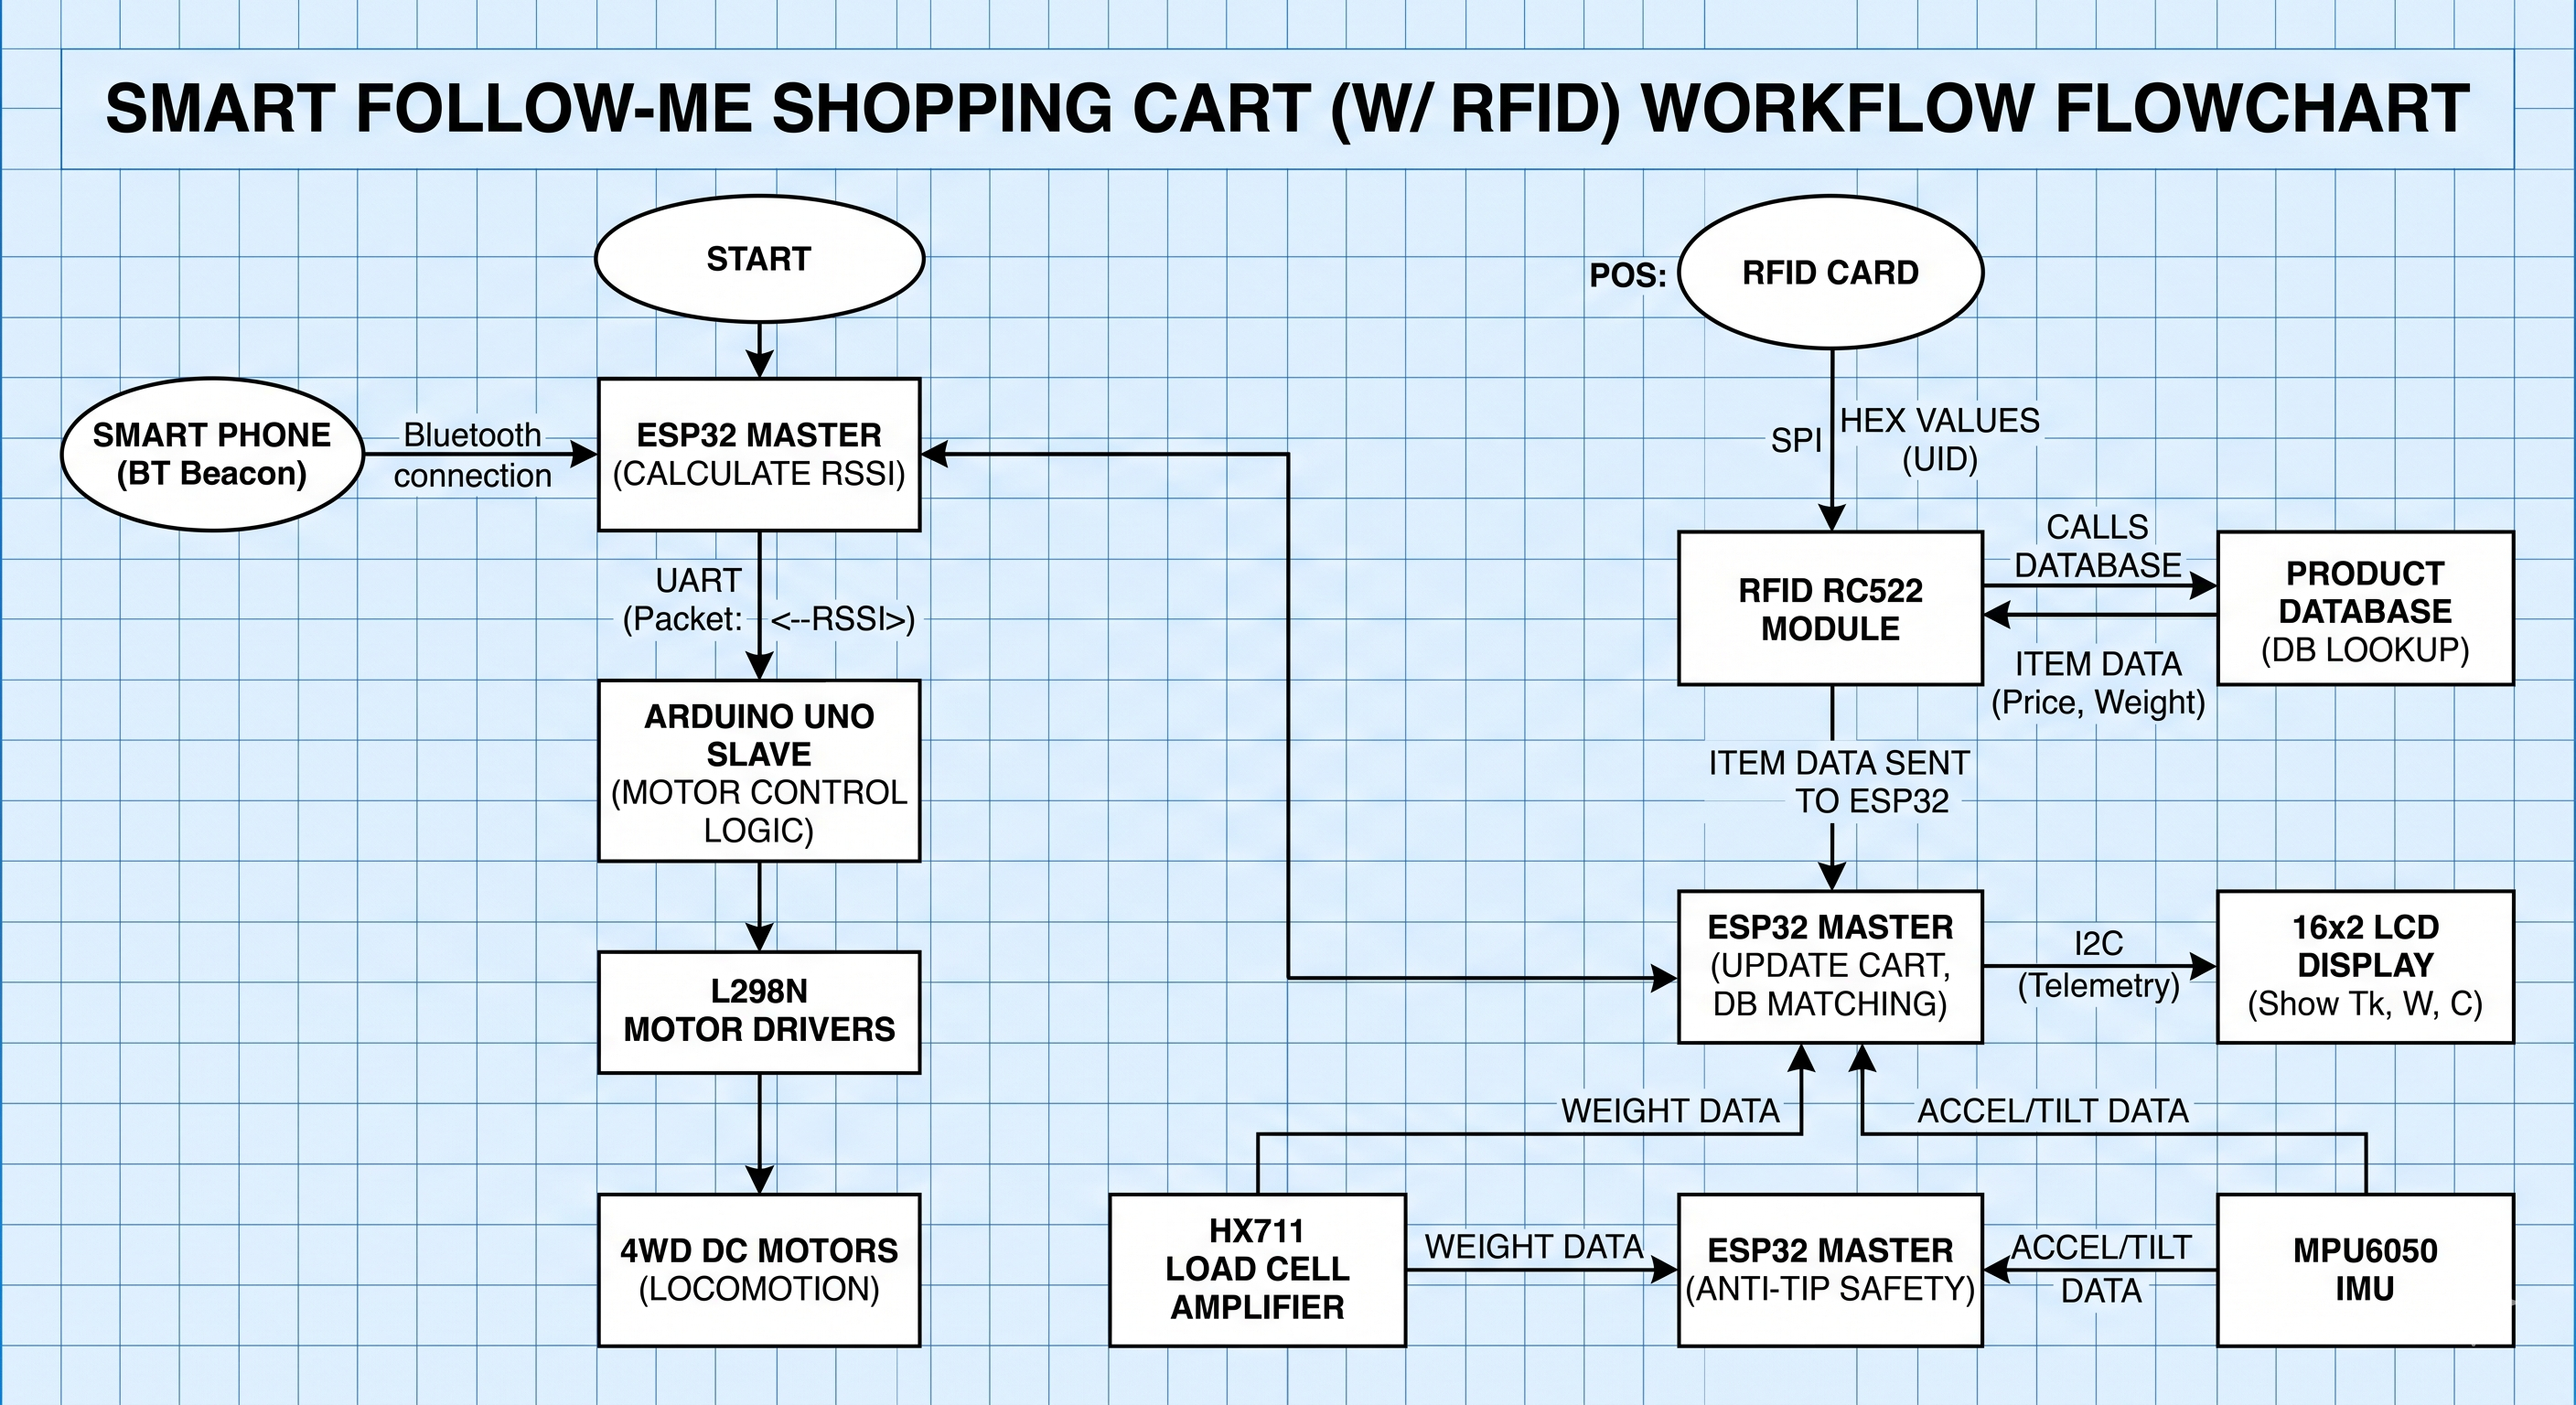
\includegraphics[width=1\linewidth]{images/workflow.png}
    \caption{Functional Workflow}
    \label{fig:workflow}
\end{figure}

\subsection{Challenges}
\begin{itemize}
    \item \textbf{ESP32-Arduino UNO Failed I2C Protocol:} ESP32 and Arduino UNO moving at different speeds caused a failure in establishing I2C Protocol between them.

    \textit{Resolution:} The protocol was changed to UART where framed data packets (e.g., $<-75>$) were transmitted at a controlled 10Hz transmission rate, coupled with a 1000ms "Deadman's Switch" timeout on the UNO to catch communication drops.

    \item \textbf{Ultrasonic "Ghost" Echoes:}  The sensors occasionally gave a false-positive reading of 0, where it should have read 999cm (in other words, 0).

    \textit{Resolution:}  A powerful software filter was applied to the UNO, by virtue of which an obstacle is only validated when the distance is over 0cm and strictly under the safety threshold without taking into consideration the anomalous high-end spikes.

    \item \textbf{4WD Motor Stalling:} Early testing had shown that the rear wheels stalled or twitched, and the front wheels were spinning, as a result of insufficient current distribution to the rear wheels and incorrect placement of logic pins across the L298N channels.

    \textit{Resolution:} The drivetrain was upgraded to a dual-L298N configuration (one driver per side). The Arduino code was refactored to utilize explicit Hardware PWM pins (D5, D9) and synchronized IN1/IN2 and IN3/IN4 states to ensure parallel power delivery to both front and rear motors.

\end{itemize}

\section{Sustainability \& Impact}
\begin{itemize}
    \item \textbf{Sustainability:} The project will use rechargeability in 3.7 V Li-ion batteries, which will significantly reduce the environmental impact caused by electricity wastes compared to the disposable alkaline batteries. When not actively pursuing conserves energy and ensures the greatest operational uptime is achieved by using low-power sleep states on the ESP32 when not actively pursuing conserves energy. The ease of replacement or re-use of parts due to the modular nature of the chassis which is 4WD.
    
    \item \textbf{Benefit:} Socially speaking, this robot will help aging, physically inactive people again gain relevance to their shopping process. Economically, it assists shoppers to remain within constrained budgets by showing real-time economical adjustments.
    
    \item \textbf{Future improvements:} A further advancement to upgrade the Bluetooth RSSI tracking to Ultra-Wideband (UWB) modules to achieve centimeter accuracy. Furthermore, a localized computer vision camera, which cross-referenced the visual information with the RFID tags, would be an added theft-deterrent.

    \item \textbf{Limitations:} Bluetooth tracking is extremely vulnerable to distortion in crowded areas (ex: human bodies between signals). Vibrations which might be caused by the 4WD motors when the cart is in motion also make the load cell sensitive to vibrations, necessitating a full stop stationary cart to have a proper tear and weight cycle. 

\end{itemize}

\section{Results \& Discussion}
The Smart Follow-Me Shopping Cart was successfully tested for navigation, safety, and POS integration, proving the efficiency of the dual-microcontroller architecture.
\begin{itemize}
    \item \textbf{Tracking \& Navigation:} The cart reliably tracked the user within an optimal BLE RSSI range of -50 to -85 dBm. Signal noise from indoor interference was successfully smoothed out using a software average filter.

    \item \textbf{Obstacle Avoidance:} The subsumption control loop performed flawlessly. The cart executed instant stops for frontal obstacles (<30 cm) and smooth "nudges" away from side obstacles (<20 cm), completely ignoring false "ghost" echoes like values of 999 cm.

    \item \textbf{POS \& Payload Verification:} RFID tag scanning was instantaneous and 100\% accurate. The load cell unfortunately developed errors which lead to rising weight with each passing moment, as such the anti-theft feature wasn’t implemented. The 3 buttons (Remove, Reset, and Checkout) instantaneously stop the robot in motion and perform as advertised.

    \item \textbf{Safety Failsafes:} System-critical safety measures successfully protected the cart during edge cases. The IMU triggered an instant lock when tilted past 35°, and the 1000ms "Deadman's Switch" successfully cut all motor power when serial communication was intentionally dropped. 
\end{itemize}

\section{Future Works}
While the current prototype successfully demonstrates the viability of an autonomous, self-checkout cart, several technical upgrades would drastically improve its commercial scalability:
\begin{itemize}
    \item \textbf{Ultra-Wideband (UWB) Integration:} To overcome the signal jitter and human-body interference inherent to BLE, future iterations will replace Bluetooth tracking with Ultra-Wideband (UWB) modules. UWB's time-of-flight (ToF) calculations will provide highly stable, centimeter-level tracking accuracy, even in dense, dynamic environments.

    \item \textbf{Anti-Theft Computer Vision:} To create a highly robust security system, RFID data could be cross-referenced with a visual profile of the item. A localized camera module (such as an ESP32-CAM or Raspberry Pi) running a lightweight object detection model could verify that the physical shape and color of the item placed in the cart matches the scanned RFID tag.

    \item \textbf{Dynamic Weighing \& Mechanical Dampening:} Currently, the cart must stop to accurately weigh items. Future designs will incorporate mechanical shock dampening and software-based data filtering (such as a Kalman filter) to isolate motor vibrations, allowing the load cell to accurately weigh items while the cart is in continuous motion.

    \item \textbf{Enhanced Navigation (SLAM):}  A 2D LiDAR scanner would upgrade the sensory array and enable the cart to use Simultaneous Localization and Mapping (SLAM). This changes the carting method of reactive obstacle braking to proactive path-planning, enabling it to smoothly negotiate the complex store layouts and moving crowds.

    \item \textbf{Omnidirectional Drivetrain:} The implementation of the Mecanum wheels in place of regular wheels would enable the cart to strafe in all directions, greatly improving its ability to manoeuvre through narrow retail shelves.

    \item \textbf{Smart Store App Integration:} The creation of a companion mobile app would enable users to input list of groceries beforehand. The app could communicate with the database of the digital layout of the store actively guiding the cart and the user along the most efficient path to desired items.
\end{itemize}

\section{Real-World Applications}
The extreme cost-effectiveness and modularity of this system enable it to expand not only of typical supermarkets but also of a wide variety of industries.

\begin{itemize}
    \item \textbf{Accessible Retail for the Disabled \& Elderly:} The main social use of this cart is to take the physical strain out of pushing heavy loads, as well as standing in long cashier lines, and provide a very accessible and dignified shopping experience to those with less mobility.

    \item \textbf{Smart Retail for SMEs:} Small to Medium Enterprises (SMEs) cannot afford the enormous costs in infrastructural costs that come with ceiling-mounted camera networks and server banks that would be required in systems such as the Amazon Dash Cart. This low-cost, localized cart helps smaller stores provide automated, cashierless check-outs without having to remodel their stores.

    \item \textbf{Warehousing \& Logistics:} The cart in fulfillment centers can serve as a follow-me autonomous helper. It dramatically reduces physical fatigue and improves logistical efficiency by transporting heavy picked orders, and floor workers.

    \item \textbf{Library \& Archival Assistance:} Often librarians are required to move bulky stacks of books using narrow corridors. A specialised adaptation of this cart might follow the staff down library stacks, carrying the physical load of this cart, but digitally recording the inventory by the built-in RFID system.

    \item \textbf{Healthcare \& Hospital Logistics:} The cart can be used to securely transport heavy medical payload, equipment, or patient charts, in medical settings. Following a BLE/UWB beacon that a nurse or doctor is carrying, the cart accepts the physical transportation of supplies and lets a nurse or doctor focus their full attention on the treatment of patients.

\end{itemize}

\newpage

\section{Conclusion}
In a nutshell, the Smart Follow-Me Shopping Cart was successfully constructed and implemented on a low cost of 4900 BDT. Once sensor fusion (Ultrasonics, IMU) was smoothly blended with the IoT technologies (ESP32, RFID, BLE), the system was equipped with its main goals: autonomous tracking, strong avoidance of collision, and easy self-service checkout system. In the testing phase, some minor environmental effects were disclosed, including: Bluetooth RSSI signal noise and load cell sensitivity to chassis vibration; the project sheds light on as a very viable and scalable concept verification. This system, however, ultimately exhibits immense potential to transform the retail sector through the promotion of freedom of consumer, the elimination of checkout lines and the achievement of distinctly obtainable shopping skills in consumers with physical disabilities.

\section{Contribution}

\small
\begin{longtable}{|p{3cm}|l|p{4cm}|p{6cm}|}
    \hline
    \textbf{Name} & \textbf{ID} & \textbf{Role/Responsibilities} & \textbf{Specific Contributions} \\
    \hline
    \endfirsthead
    
    % This section repeats the header on the next page if the table breaks
    \hline
    \textbf{Name} & \textbf{ID} & \textbf{Role/Responsibilities} & \textbf{Specific Contributions} \\
    \hline
    \endhead
    
    Fariha Tanha & 22101296 & Co-Integrator, Crafter, Implement BLE  & Developed the autonomous tracking system using Bluetooth signal (IOS App: Lightblue), Implemented I2C communication to connect the LCD display and the MPU to the ESP32, Manually built the custom diy cart box with specific measurements. \\
    \hline
    
    Mohammad Jabir Safa Khandoker & 22201108 & Project Lead, Code Developer, Component Buyer, Solderer & Wrote all the code for both Arduino UNO and ESP32, Planned and bought all required components, Implemented Master-Slave configuration between ESP32 \& Arduino UNO, Soldered required components for better conduction \\
    \hline
    
    Aarya Ibteda Foyez & 22201509 & Integrated RFID with the Robot & Raw RFID bytes are normalized into their corresponding consistent Hex strings by an ESP32 formatting loop to obtain consistent identifications, Engineered a Weight-Verifying  RFID Scanner utilizing MFRC522 RFID reader and an HX711 load cell, Installed automated validation logic to prove that the scanned UIDs equaled the actual weight of items, Created a Virtual Cart and billing integration with Arduino style C++ directly upon the ESP32. \\
    \hline
    
    Mugdha Farheen Kibria & 22299206 & Co-Integrator, Sensor Logic Developer (Sonar \& Load Cell), Poster & Wired and configured HC-SR04 ultrasonic sensors with the Arduino UNO for obstacle detection, Programmed data filters in the Arduino code to stabilise sonar readings and prevent erratic braking, Wired and calibrated the 10kg load cell with the HX711 amplifier for the weighing mechanism, Troubleshooting hardware and sensor drift issues during system testing. \\
    \hline
    
    Safwan Masud & 23101425 & Hardware/ Mechanical Assembly and Motor Driver System Setup, Secondary Component Buyer & Put together the 4WD chassis and cart frame, ensuring that it was sturdy and strong enough, Fitted all the DC gear motors to the chassis, fitted the wheels, and made sure proper alignment was maintained in order to move freely, Both L298N driver modules were wired and configured, Involved in the procurement of extra components needed later on. \\
    \hline
\end{longtable}

\section*{References}
\begin{enumerate}
    \item Technology Guide5. (2021, June 18). Arduino 4WD Robot Car Kit unboxing \& assembling process | Arduino car chassis [Video]. YouTube. \url{https://www.youtube.com/watch?v=alJiBayh1To}
\end{enumerate}

\end{document}
